\section*{ÔN TẬP CHƯƠNG VIII}
\subsection{Bài tập trắc nghiệm}
\Opensolutionfile{ans}[ans/KNTT-Tap2-BT-CuoiChuong-VII]
\begin{ex}%[1K7BO-1]
	Cho các phát biểu sau:
	\begin{itemize}
	\item Hai mặt phẳng $(P)$ và $(Q)$ có giao tuyến là đường thẳng $a$ và cùng vuông góc với mặt phẳng $(R)$ thì $a\perp(R)$.
	\item Hai mặt phẳng $(P)$ và $(Q)$ vuông góc với nhau và có giao tuyến là đường thẳng $a$, một đường thẳng $b$ nằm trong mặt phẳng $(P)$ và vuông góc với đường thẳng $a$ thì $b\perp(Q)$.
	\item Mặt phẳng $(P)$ chứa đường thẳng $a$ và $a$ vuông góc với $(Q)$ thì $(P)\perp(Q)$.
	\item Đường thẳng $a$ nằm trong mặt phẳng $(P)$ và mặt phẳng $(P)$ vuông góc với mặt phẳng $(Q)$ thì $a\perp(Q)$.
	\end{itemize}
	Số phát biểu đúng trong các phát biểu trên là
	\choice
	{$1$}
	{$2$}
	{\True $3$}
	{$4$} 
	\loigiai{
	Mệnh đề 1, 2, 3 đúng. Mệnh đề 4 sai.
	}
\end{ex}
\begin{ex}%[1K7BO-1]
	Cho mặt phẳng $(P)$ vuông góc với mặt phẳng $(Q)$ và $a$ là giao tuyến của $(P)$ và $(Q)$. Trong các phát biểu dưới đây, phát biểu nào đúng?
	\choice
	{Đường thẳng $d$ nằm trên $(Q)$ thì $d$ vuông góc với $(P)$}
	{\True Đường thẳng $d$ nằm trên $(Q)$ và $d$ vuông góc với $a$ thì $d$ vuông góc với $(P)$}
	{Đường thẳng $d$ vuông góc với $a$ thì $d$ vuông góc với $(P)$}
	{Đường thẳng $d$ vuông góc với $(Q)$ thì $d$ vuông góc với $(P)$}
	\loigiai{}
\end{ex}
\begin{ex}%[1K7YO-7]
	Thể tích của khối chóp có diện tích đáy bằng $\mathbf{S}$, chiều cao bằng $h$ là
	\choice
	{$V=\mathbf{S}\cdot h$}
	{$V=\dfrac{1}{2}\mathbf{S}\cdot h$}
	{\True $V=\dfrac{1}{3}\mathbf{S}\cdot h$}
	{$V=\dfrac{2}{3}\mathbf{S}\cdot h$}
	\loigiai{}
\end{ex}
\begin{ex}%[1C8Y6-2]
	Cho khối lăng trụ có diện tích đáy bằng $a^2$ và chiều cao bằng $3a$. Thể tích của khối lăng trụ đó bằng
	\choice
	{$a^3$}
	{\True $3a^3$}
	{$\dfrac{a^3}{3}$}
	{$9a^3$}
	\loigiai{
	Thể tích khối lăng trụ đó bằng $a^2\cdot 3a=3a^3$.
	}
\end{ex}
\begin{ex}%[1C8Y6-2]
	Cho khối chóp có diện tích đáy là $a^2$ và chiều cao là $3a$. Thể tích của khối chóp bằng
	\choice
	{\True $a^3$}
	{$3a^3$}
	{$\dfrac{a^3}{3}$}
	{$9a^3$}
	\loigiai{
	Thể tích của khối chóp bằng $\dfrac{1}{3}\cdot a^2\cdot 3a=a^3$.
	}
\end{ex}
\begin{ex}%[1K7KO-4]
	Cho hình chóp tứ giác đều $S.ABCD$. Phát biểu nào sau đây là đúng?
	\choice
	{Số đo của góc nhị diện $[S, AB, C]$ bằng $\widehat{SBC}$}
	{Số đo của góc nhị diện $[D, SA, B]$ bằng $90^{\circ}$}
	{\True Số đo của góc nhị diện $[S, AC, B]$ bằng $90^{\circ}$}
	{Số đo của góc nhị diện $[D, SA, B]$ bằng $\widehat{BSD}$} 
	\loigiai{
	\immini{
	Gọi $O =AC \cap BD$.
	Ta có $SO \perp (ABCD)$ do $S.ABCD$ là hình chóp đều.\\
	Mà $SO \subset (SAC)$ nên $(SAC) \perp (ABCD).$\\
	Suy ra, số đo của góc nhị diện $[S, AC, B]$ bằng $90^{\circ}$.
	}
	{
	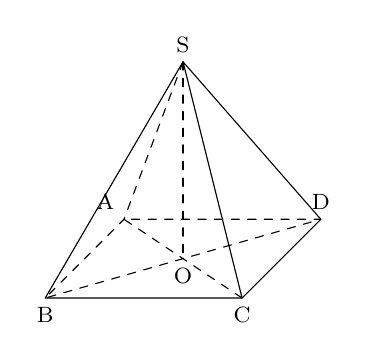
\begin{tikzpicture}[line join=round,line cap=round,>=stealth,font=\footnotesize,scale=0.5]
	\coordinate [label=above left:A] (A) at (-5,-2);
	\coordinate [label=below:B](B) at (-7,-4);
	\coordinate [label=below:C] (C) at (-2,-4);
	\coordinate [label=above:D] (D) at (0,-2);
	\coordinate [label=above:S] (S) at (-3.5,2);
	\coordinate [label=below:O] (O) at (-3.5,-3);
	\draw (S)--(B)--(C)--(D)--(S)--(C);
	\draw[dashed] (S)--(A)--(B)--(D)--(A)--(C);
	\draw[dashed] (S)--(O);
	\end{tikzpicture}
	}
	}
\end{ex}
\begin{ex}% [1K7BO-2]
	Cho hình chóp $S.ABCD$ có đáy $ABCD$ là hình vuông và $SA\perp(ABCD)$.
	Phát biểu nào sau đây là \textbf{sai}?
	\choice
	{$BC\perp (SAB)$}
	{$BD\perp (SAC)$}
	{\True $AC\perp (SBD)$}
	{$AD\perp (SAB)$} 
	\loigiai{
	\immini{
	Gọi $O = AC \cap BD$.\\
	Do $SA \perp (ABCD) $ nên $SA \perp AO \Rightarrow \Delta SAO$ vuông tại $A$.\\
	Do đó, $AC$ không thể vuông góc với $SO$. Vậy, $AC$ không thể vuông góc với mặt phẳng $(SBD).$
	}
	{
	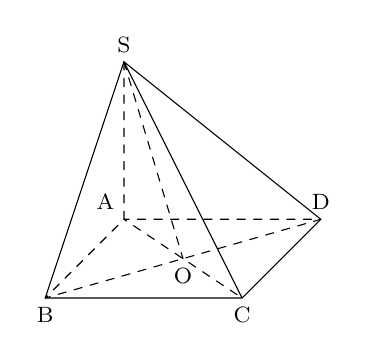
\begin{tikzpicture}[line join=round,line cap=round,>=stealth,font=\footnotesize,scale=0.5]
	\coordinate [label=above left:A] (A) at (-5,-2);
	\coordinate [label=below:B](B) at (-7,-4);
	\coordinate [label=below:C] (C) at (-2,-4);
	\coordinate [label=above:D] (D) at (0,-2);
	\coordinate [label=above:S] (S) at (-5,2);
	\coordinate [label=below:O] (O) at (-3.5,-3);
	\draw (S)--(B)--(C)--(D)--(S)--(C);
	\draw[dashed] (S)--(A)--(B)--(D)--(A)--(C);
	\draw[dashed] (S)--(O);
	\end{tikzpicture}
	}
	}
\end{ex}
\begin{ex}%[1T8B2-2]
	\immini{Cho hình chóp $S.ABCD$ có đáy $ABCD$ là hình vuông, $SA$ vuông góc với mặt đáy. Đường thẳng $CD$ vuông góc với mặt phẳng nào sau đây?
	\choice
	{\True $(SAD)$}
	{$(SAC)$}
	{$(SAB)$}
	{$(SBD)$}
	}{\begin{tikzpicture}[scale=0.6, font=\footnotesize, line join=round, line cap=round, >=stealth]
	\def\bc{4} % cạnh BC
	\def\ba{2} % cạnh BA
	\def\h{4} % đường cao
	\def\gocB{30} % góc B của đáy
	\coordinate[label=below left:$B$] (B) at (0,0);
	\coordinate[label=above left:$A$] (A) at (\gocB:\ba);
	\coordinate[label=below:$C$] (C) at (\bc,0);
	\coordinate[label=right:$D$] (D) at ($(C)-(B)+(A)$);
	\coordinate[label=above:$S$] (S) at ($(A)+(90:\h)$);
	\draw[thick] (B)--(C)--(D)--(S)--cycle (S)--(C);
	\draw[dashed] (A)--(D) (S)--(A)--(B);
	\foreach \diem in {A,B,C,D,S}	\fill (\diem)circle(1.5pt);
	\newcommand{\gocv}[4][black]{\draw[#1] ($(#3)!5pt!(#2)$)--($(#3)!2!($($(#3)!5pt!(#2)$)!.5!($(#3)!5pt!(#4)$)$)$)--($(#3)!5pt!(#4)$);}
	\gocv{S}{A}{D}
	\end{tikzpicture}
	}
	\loigiai{Ta có $\heva{&CD \perp AD\\&CD \perp SA\\&SA \cap AD = \{A\}\\&SA, AD \subset (SAD)} \Rightarrow CD \perp (SAD)$.
	}
\end{ex}
\begin{ex}%[1T8B5-1]
	\immini{Cho hình chóp $S.ABCD$ có đáy $ABCD$ là hình vuông cạnh $b$, $SA$ vuông góc với mặt đáy, $SC = 2b\sqrt{2}$. Số đo góc giữa cạnh bên $SC$ và mặt đáy là
	\choice
	{$60^\circ$}
	{$30^\circ$}
	{$45^\circ$}
	{$50^\circ$}
	}{\begin{tikzpicture}[scale=0.65, font=\footnotesize, line join=round, line cap=round, >=stealth]
	\def\bc{4} % cạnh BC
	\def\ba{2} % cạnh BA
	\def\h{4} % đường cao
	\def\gocB{30} % góc B của đáy
	\coordinate[label=below left:$B$] (B) at (0,0);
	\coordinate[label=above left:$A$] (A) at (\gocB:\ba);
	\coordinate[label=below:$C$] (C) at (\bc,0);
	\coordinate[label=right:$D$] (D) at ($(C)-(B)+(A)$);
	\coordinate[label=above:$S$] (S) at ($(A)+(90:\h)$);
	\draw[thick] (B)--(C)--(D)--(S)--cycle (S)--(C);
	\draw[dashed] (A)--(D) (S)--(A)--(B);
	\foreach \diem in {A,B,C,D,S}	\fill (\diem)circle(1.5pt);
	\newcommand{\gocv}[4][black]{\draw[#1] ($(#3)!5pt!(#2)$)--($(#3)!2!($($(#3)!5pt!(#2)$)!.5!($(#3)!5pt!(#4)$)$)$)--($(#3)!5pt!(#4)$);}
	\gocv{S}{A}{D}
	\end{tikzpicture}
	}
	\loigiai{
	\immini{Do $SA \perp (ABCD)$ nên $AC$ là hình chiếu của $SC$ trên $(ABCD)$.\\
	Suy ra $(SC,(ABCD)) = (SC,AC) = \widehat{SCA}$.\\
	Trong $\triangle SAC$ vuông tại $A$ với $AC = b\sqrt{2}$, $SC = 2b\sqrt{2}$ có
	\[\cos \widehat{SCA} = \dfrac{AC}{SC} = \dfrac{b\sqrt{2}}{2b\sqrt{2}} = \dfrac{1}{2} \Rightarrow \widehat{SCA} = 60^\circ.\]
	}{\begin{tikzpicture}[scale=0.65, font=\footnotesize, line join=round, line cap=round, >=stealth]
	\def\bc{4} % cạnh BC
	\def\ba{2} % cạnh BA
	\def\h{4} % đường cao
	\def\gocB{30} % góc B của đáy
	\coordinate[label=below left:$B$] (B) at (0,0);
	\coordinate[label=above left:$A$] (A) at (\gocB:\ba);
	\coordinate[label=below:$C$] (C) at (\bc,0);
	\coordinate[label=right:$D$] (D) at ($(C)-(B)+(A)$);
	\coordinate[label=above:$S$] (S) at ($(A)+(90:\h)$);
	\draw[thick] (B)--(C)--(D)--(S)--cycle (S)--(C);
	\draw[dashed] (A)--(D) (S)--(A)--(B) (A)--(C);
	\foreach \diem in {A,B,C,D,S}	\fill (\diem)circle(1.5pt);
	\draw pic[draw,black,angle radius=4mm] {angle = S--C--A} ($($(C)!4mm!(A)$)!.6!($(C)!13mm!(S)$)$)node[rotate=0]{};
	\newcommand{\gocv}[4][black]{\draw[#1] ($(#3)!5pt!(#2)$)--($(#3)!2!($($(#3)!5pt!(#2)$)!.5!($(#3)!5pt!(#4)$)$)$)--($(#3)!5pt!(#4)$);}
	\gocv{S}{A}{D}
	\end{tikzpicture}
	}
	}
\end{ex}
\begin{ex}%[1T8K4-3]
	Cho hình chóp tam giác đều $S.ABC$ có cạnh đáy bằng $2a$ và chiều cao bằng $a\sqrt{2}$. Khoảng cách từ tâm $O$ của đáy $ABC$ đến một mặt bên là
	\choice
	{\True $\dfrac{a\sqrt{14}}{7}$}
	{$\dfrac{a\sqrt{2}}{7}$}
	{$\dfrac{a\sqrt{14}}{2}$}
	{$\dfrac{2a\sqrt{14}}{7}$}
	\loigiai{
	\immini{Gọi $M$ là trung điểm $BC$ và $O$ là trọng tâm $\triangle ABC$.\\
	Khi đó $AM \perp BC$ và $SO \perp (ABC)$.\\
	Gọi $H$ là hình chiếu của $O$ trên $SM$\\
	Ta có $\heva{&BC \perp AM\\&BC \perp SO\\&SO, AM \subset (SAM)\\&SO \cap AM = \{O\}} \Rightarrow BC \perp (SAM) \Rightarrow BC \perp OH$.\\
	Vậy $OH \perp (SBC)$. Suy ra $\mathrm{\,d}(O,(SBC)) = OH$.\\
	Trong $\triangle SOM$ với $AM = \dfrac{2a\sqrt{3}}{2} = a\sqrt{3} \Rightarrow OM = \dfrac{1}{3}AM= \dfrac{a\sqrt{3}}{3}$; $SO = a\sqrt{2}$ ta có
	\[OH = \dfrac{SO \cdot OM}{\sqrt{SO^2 + OM^2}} = \dfrac{a\sqrt{2} \cdot \dfrac{a\sqrt{3}}{3}}{\sqrt{(a\sqrt{2})^2 + \left(\dfrac{a\sqrt{3}}{3}\right)^2}} = \dfrac{a\sqrt{14}}{7}.\]
	}{\begin{tikzpicture}[scale=0.8, font=\footnotesize, line join=round, line cap=round, >=stealth]
	\def\ac{4} % cạnh AC
	\def\ab{2} % cạnh AB
	\def\h{4} % chiều cao
	\def\gocA{50} % góc A của đáy
	\coordinate[label=left:$A$] (A) at (0,0);
	\coordinate[label=right:$C$] (C) at (\ac,0);
	\coordinate[label=below left:$B$] (B) at (-\gocA:\ab);
	\coordinate[label=below right:$M$] (M) at ($(B)!.5!(C)$);
	\coordinate[label=below:$O$] (O) at ($(A)!2/3!(M)$);
	\coordinate[label=above:$S$] (S) at ($(O)+(90:\h)$);
	\coordinate[label=right:$H$] (H) at ($(S)!0.7!(M)$);
	\draw[thick] (A)--(B)--(C)--(S)--cycle (S)--(B) (S)--(M);
	\draw[dashed] (M)--(A)--(C) (O)--(S) (O)--(H);
	\foreach \diem in {A,B,C,S,O,M,H}	\fill (\diem)circle(1.5pt);
	\newcommand{\gocv}[4][black]{\draw[#1] ($(#3)!5pt!(#2)$)--($(#3)!2!($($(#3)!5pt!(#2)$)!.5!($(#3)!5pt!(#4)$)$)$)--($(#3)!5pt!(#4)$);}
	\gocv{A}{M}{B}
	\gocv{S}{O}{M}
	\gocv{O}{H}{M}
	\end{tikzpicture}
	}
	}
\end{ex}
\begin{ex}%[1T8B3-2]
	Cho hình chóp $S.ABCD$ có các canh bên và cạnh đáy đều bằng $a$. Gọi $M$ là trung điểm của $SA$. Mặt phẳng $(MBD)$ vuông góc với mặt phẳng nào dưới đây?
	\choice
	{$(SBC)$}
	{\True $(SAC)$}
	{$(SBD)$}
	{$(ABCD)$}
	\loigiai{
	\immini{Ta có $\heva{&SA \perp BM\\&SA \perp DM\\&BM, DM \subset (MBD)\\&BM \cap DM = \{M\}} \Rightarrow SA \perp (MBD)$ (1).\\
	Mặt khác $SA \subset (SAC)$ (2).\\
	Từ (1) và (2) suy ra $(SAC) \perp (MBD)$.
	}{\vspace*{-4mm}
	\begin{tikzpicture}[scale=0.85, font=\footnotesize, line join=round, line cap=round, >=stealth]
	\def\bc{4} % cạnh BC
	\def\ba{2} % cạnh BA
	\def\h{4} % đường cao
	\def\gocB{30} % góc B của đáy
	\coordinate[label=below left:$B$] (B) at (0,0);
	\coordinate[label=above right:$A$] (A) at (\gocB:\ba);
	\coordinate[label=below:$C$] (C) at (\bc,0);
	\coordinate[label=right:$D$] (D) at ($(C)-(B)+(A)$);
	\coordinate (O) at ($(A)!.5!(C)$);
	\coordinate[label=above:$S$] (S) at ($(O)+(90:\h)$);
	\coordinate[label=right:$M$] (M) at ($(S)!0.5!(A)$);
	\draw[thick] (B)--(C)--(D)--(S)--cycle (S)--(C);
	\draw[dashed] (C)--(A)--(D)--(B) (M)--(B) (M)--(D) (S)--(A)--(B);
	\foreach \diem in {A,B,C,D,S,M}	\fill (\diem)circle(1.5pt);
	\newcommand{\gocv}[4][black]{\draw[#1] ($(#3)!5pt!(#2)$)--($(#3)!2!($($(#3)!5pt!(#2)$)!.5!($(#3)!5pt!(#4)$)$)$)--($(#3)!5pt!(#4)$);}
	\gocv{A}{M}{D}
	\gocv{A}{M}{B}
	\end{tikzpicture}
	}
	}
\end{ex}
\begin{ex}%[1C8Y6-2]
	Cho tứ diện $OABC$ thỏa mãn $OA=a$, $OB=b$, $OC=c$, $\widehat{AOB}=\widehat{BOC}=\widehat{COA}=90^\circ$. Thể tích của khối tứ diện $OABC$ bằng
	\choice
	{$abc$}
	{$\dfrac{abc}{2}$}
	{$\dfrac{abc}{3}$}
	{\True $\dfrac{abc}{6}$}
	\loigiai{
	\immini{
	Diện tích tam giác $OBC$ là $S_{\triangle {OBC}}=\dfrac{1}{2}\cdot OB\cdot OC=\dfrac{1}{2}\cdot bc$.\\
	Thể tích của khối tứ diện $OABC$ là $V_{OABC}=\dfrac{1}{3}\dot S_{\triangle {OBC}}\cdot OA=\dfrac{abc}{6}$.
	}{
	\begin{tikzpicture}[scale=1, font=\footnotesize, line join=round, line cap=round, >=stealth]
	\path
	(0,0) coordinate (O)
	(-1,-1) coordinate (B)
	(3,0) coordinate (C)
	($(O)+(0,2.5)$) coordinate (A)
	;
	\draw (A)--(B)--(C)--(A);
	\draw[dashed] (O)--(A) (O)--(B) (O)--(C);
	\foreach \x/\g in {O/170,A/90,B/-120,C/0} \draw[fill=black] (\x) circle(1pt)++(\g:0.3)node{$\x$};
	\draw pic[draw=black, angle eccentricity=2, angle radius=0.25cm]{right angle=C--O--A};
	\draw pic[draw=black, angle eccentricity=2, angle radius=0.25cm]{right angle=A--O--B};
	\draw pic[draw=black, angle eccentricity=2, angle radius=0.25cm]{right angle=B--O--C};
	\end{tikzpicture}
	}
	}
\end{ex}
\begin{ex}%[1T8K5-2]
	Cho chóp tứ giác $S.ABCD$ có đáy là hình chữ nhật với $AB = 4a$, $AD = 3a$. Các cạnh bên đều có độ dài $5a$. Góc nhị diện $[S, BC, A]$ có số đo là
	\choice
	{$75^\circ 46'$}
	{$71^\circ 21'$}
	{$68^\circ 31'$}
	{\True $65^\circ 12'$}
	\loigiai{
	\immini{Gọi $O$ là tâm hình chữ nhật $ABCD$.\\
	$\triangle SAC$, $\triangle SBD$ đều là các tam giác cân tại $S$ nên suy ra $SO \perp (ABCD)$.\\
	Ta có $OM \perp BC$, $SM \perp BC$ nên suy ra góc nhị diện $[S, BC, A]$ là $\widehat{SMO}$.\\
	Trong $\triangle SMO$ vuông tại $O$ với $OM = \dfrac{AB}{2} = 2a$,\\ $SM = \sqrt{SC^2 - MC^2} = \sqrt{25a^2 - \dfrac{9a^2}{4}} = \dfrac{a\sqrt{91}}{2}$.\\
	Ta có $\cos \widehat{SMO} = \dfrac{OM}{SM} = \dfrac{2a}{\dfrac{a\sqrt{91}}{2}} = \dfrac{4\sqrt{91}}{91} \Rightarrow \widehat{SMO} \approx 65^\circ 12'31{,}39''$.
	}{\begin{tikzpicture}[scale=0.8, font=\footnotesize, line join=round, line cap=round, >=stealth]
	\def\bc{4} % cạnh BC
	\def\ba{2} % cạnh BA
	\def\h{4} % đường cao
	\def\gocB{30} % góc B của đáy
	\coordinate[label=below left:$B$] (B) at (0,0);
	\coordinate[label=above left:$A$] (A) at (\gocB:\ba);
	\coordinate[label=below:$C$] (C) at (\bc,0);
	\coordinate[label=right:$D$] (D) at ($(C)-(B)+(A)$);
	\coordinate[label=above right:$O$] (O) at ($(A)!.5!(C)$);
	\coordinate[label=above:$S$] (S) at ($(O)+(90:\h)$);
	\coordinate[label=below:$M$] (M) at ($(B)!.5!(C)$);
	\draw[thick] (B)--(C)--(D)--(S)--cycle (S)--(C) (S)--(M);
	\draw[dashed] (C)--(A)--(D)--(B) (O)--(S)--(A)--(B) (O)--(M);
	\foreach \diem in {A,B,C,D,S,O,M}	\fill (\diem)circle(1.5pt);
	\draw pic[draw,black,angle radius=2.5mm] {angle = O--M--S} ($($(M)!4mm!(S)$)!.6!($(M)!13mm!(O)$)$)node[rotate=0]{};
	\end{tikzpicture}
	}
	}
\end{ex}
\begin{ex}%[1T8B4-7]
	Thể tích của khối chóp cụt tam giác đều có cạnh đáy lớn bằng $2a$, cạnh đáy nhỏ bằng $a$ và chiều cao bằng $\dfrac{a\sqrt{6}}{3}$ là
	\choice
	{$\dfrac{7\sqrt{2}}{8} a^3$}
	{$\dfrac{\sqrt{2}}{4} a^3$}
	{\True $\dfrac{7\sqrt{2}}{12} a^3$}
	{$\dfrac{7\sqrt{3}}{4} a^3$}
	\loigiai{
	\immini{Gọi $H$ và $H'$ lần lượt là tâm đáy $ABC$ và $A'B'C'$.\\
	Suy ra $HH' = \dfrac{a\sqrt{6}}{3}$.\\
	Diện tích $\triangle ABC$ là $S = \dfrac{4a^2\sqrt{3}}{4} = a^2\sqrt{3}$ (đvtt).\\
	Diện tích $\triangle A'B'C'$ là $S = \dfrac{a^2\sqrt{3}}{4}$ (đvtt).\\
	Vậy thể tích của khối chóp cụt $ABC.A'B'C'$ là
	\allowdisplaybreaks
	\begin{eqnarray*}
	V &=& \dfrac{1}{3} HH'(S + \sqrt{SS'} + S')\\
	&=&\dfrac{1}{3} \cdot \dfrac{a\sqrt{6}}{3}\left(a^2\sqrt{3} + \sqrt{a^2\sqrt{3} \cdot \dfrac{a^2\sqrt{3}}{4}} + \dfrac{a^2\sqrt{3}}{4}\right)\\
	&=& \dfrac{7\sqrt{2}}{12} a^3.
	\end{eqnarray*}
	}{\begin{tikzpicture}[scale=1, font=\footnotesize, line join=round, line cap=round, >=stealth]
	\tkzInit[xmin=-1,xmax=5.5,ymin=-2.5, ymax=2.7] \tkzClip[space=.1]
	\tkzDefPoints{0/0/A,5/0/C,2/-1.5/B,0/5/x}
	\coordinate (I) at ($(B)!0.5!(C)$);
	\coordinate (H) at ($(A)!2/3!(I)$);
	\coordinate (S) at ($(H)+(x)$);
	\coordinate (A') at ($(S)!0.5!(A)$);
	\coordinate (B') at ($(S)!0.5!(B)$);
	\coordinate (C') at ($(S)!0.5!(C)$);
	\coordinate (H') at ($(S)!0.5!(H)$);
	\coordinate (M) at ($(H)-(H')+(A')$);
	\tkzDrawSegments(A,B B,C C,C' B,B' A,A' A',B' B',C' C',A' A',H')
	\tkzDrawSegments[dashed](A,C H,H' A,H)
	\foreach \x/\g in {A/180,B/-90,C/0,A'/150,C'/30,B'/-150,H/-60,H'/0} \fill[black] (\x) circle (1pt) +(\g:0.3)node{$\x$};
	\end{tikzpicture}
	}
	}
\end{ex}
\begin{ex}%[1T8B3-6]
	Nếu hình hộp chữ nhật có ba kích thước là $3$; $4$; $5$ thì độ dài đường chéo của nó là
	\choice
	{$5\sqrt{2}$}
	{$50$}
	{$2\sqrt{5}$}
	{$12$}
	\loigiai{
	\immini{Cho hình hộp chữ nhật $ABCD.A'B'C'D'$ với $AB = 3$; $AD = 4$; $AA' = 5$.\\
	Ta có $AC = \sqrt{AB^2 + AD^2} = \sqrt{3^2 + 4^2} = 5$.\\
	Suy ra $A'C = \sqrt{AA'^2 + AC^2} = \sqrt{5^2 + 5^2} = 5\sqrt{2}$.
	}{\begin{tikzpicture}[scale=0.5, font=\footnotesize, line join=round, line cap=round, >=stealth]
	\def\bc{5} % cạnh BC
	\def\ba{3} % cạnh BA
	\def\h{4} % đường cao
	\def\gocB{35} % góc B của đáy
	\coordinate[label=below left:$B$] (B) at (0,0);
	\coordinate[label=above left:$A$] (A) at (\gocB:\ba);
	\coordinate[label=below:$C$] (C) at (\bc,0);
	\coordinate[label=right:$D$] (D) at ($(C)-(B)+(A)$);
	\coordinate[label=above left:$A'$] (A') at ($(A)+(90:\h)$);
	\coordinate[label=left:$B'$] (B') at ($(B)-(A)+(A')$);
	\coordinate[label=below right:$C'$] (C') at ($(C)-(A)+(A')$);
	\coordinate[label=right:$D'$] (D') at ($(D)-(A)+(A')$);
	\draw[thick] (B')--(B)--(C)--(D)--(D')--(A')--(B')--(C')--(D') (C)--(C') (A')--(C');
	\draw[dashed] (A')--(A)--(D) (A)--(B) (A')--(C) (A)--(C);
	\foreach \diem in {A,B,C,D,A',B',C',D'}	\fill (\diem)circle(1.5pt);
	\end{tikzpicture}
	}
	}
\end{ex}
\begin{ex}%[1T8B4-6]
	Thể tích của khối lăng trụ tam giác đều có tất cả các cạnh đều bằng $a$ là
	\choice
	{\True $\dfrac{a^3\sqrt{3}}{4}$}
	{$\dfrac{a^3\sqrt{3}}{3}$}
	{$\dfrac{a^3\sqrt{2}}{3}$}
	{$\dfrac{a^3\sqrt{2}}{2}$}
	\loigiai{
	\immini{Ta có $S_{\triangle ABC} = \dfrac{a^2\sqrt{3}}{4}$.\\
	Vậy thể tích khối lăng trụ $ABC.A'B'C'$ là $$V = S_{\triangle ABC} \cdot AA' = \dfrac{a^2\sqrt{3}}{4} \cdot a = \dfrac{a^3\sqrt{3}}{4} \;\;\text{(đvtt).}$$ 
	}{\begin{tikzpicture}[scale=0.6, font=\footnotesize, line join=round, line cap=round, >=stealth]
	\def\ac{4} % cạnh AC
	\def\ab{2} % cạnh AB
	\def\h{4} % chiều cao
	\def\gocA{50} % góc A của đáy
	\coordinate[label=left:$A$] (A) at (0,0);
	\coordinate[label=right:$C$] (C) at (\ac,0);
	\coordinate[label=below left:$B$] (B) at (-\gocA:\ab);
	\coordinate[label=left:$A'$] (A') at ($(A)+(90:\h)$);
	\coordinate[label=below left:$B'$] (B') at ($(B)-(A)+(A')$);
	\coordinate[label=right:$C'$] (C') at ($(C)-(A)+(A')$);
	\draw[thick] (A')--(A)--(B)--(C)--(C')--(A')--(B')--(C') (B)--(B');
	\draw[dashed] (A)--(C);
	\foreach \diem in {A,B,C,A',B',C'} \fill (\diem)circle(1.5pt);
	\end{tikzpicture}
	}
	}
\end{ex}
\begin{ex}%[1C8Y6-1]
	Cho hình lập phương $MNPQ.M'N'P'Q'$ có cạnh bằng $a$. Góc giữa hai đường thẳng $MN$ và $M'P'$ bằng
	\choice
	{$30^\circ$}
	{\True $45^\circ$}
	{$60^\circ$}
	{$90^\circ$}
	\loigiai{
	\immini{
	Ta có $MP\parallel M'P'$ nên $(MN,M'P')=(MN,MP)=\widehat{NMP}=45^\circ$.
	}{
	\begin{tikzpicture}[scale=0.8, font=\footnotesize, line join=round, line cap=round, >=stealth]
	\path
	(0,0) coordinate (M)
	(-1,-1) coordinate (N)
	(3,0) coordinate (Q)
	($(N)+(Q)-(M)$) coordinate (P)
	($(M)+(0,2.5)$) coordinate (M')
	($(M')-(M)+(N)$) coordinate (N')
	($(M')-(M)+(P)$) coordinate (P')
	($(M')-(M)+(Q)$) coordinate (Q')
	;
	\draw (M')--(N')--(P')--(Q')--(M') (N)--(N') (P)--(P') (Q)--(Q') (N)--(P)--(Q) (M')--(P');
	\draw[dashed] (M')--(M)--(N) (M)--(Q) (M)--(P);
	\foreach \x/\g in {M/180,N/-90,P/-90,Q/0,M'/90,N'/180,P'/90,Q'/0} \draw[fill=black] (\x) circle(1pt)++(\g:0.3)node{$\x$};
	\draw pic["$45^\circ$",draw=black, angle eccentricity=2, angle radius=0.25cm]{angle=N--M--P};
	\end{tikzpicture}
	}
	}
\end{ex}
\begin{ex}%[1C8Y6-1]
	Cho hình lập phương $MNPQ.M'N'P'Q'$ có cạnh bằng $a$. Gọi $\alpha$ là số đo góc giữa đường thẳng $M'P$ và mặt phẳng $(MNPQ)$. Giá trị $\tan \alpha$ bằng
	\choice
	{$1$}
	{$2$}
	{$\sqrt{2}$}
	{\True $\dfrac{1}{\sqrt{2}}$}
	\loigiai{
	\immini{
	Ta có $MM'\perp (MNPQ)$ nên $MP$ là hình chiếu vuông góc của $M'P$ lên $(MNPQ)$.\\
	Do đó góc giữa đường thẳng $M'P$ và mặt phẳng $(MNPQ)$ là $(M'P,MP)=\widehat{M'PM}=\alpha$.\\
	Lại có $MM'=a$, $MP=a\sqrt{2}$ nên $$\tan \alpha=\tan \widehat{M'PM}=\dfrac{MM'}{MP}=\dfrac{1}{\sqrt{2}}.$$
	}{
	\begin{tikzpicture}[scale=0.8, font=\footnotesize, line join=round, line cap=round, >=stealth]
	\path
	(0,0) coordinate (M)
	(-1,-1) coordinate (N)
	(3,0) coordinate (Q)
	($(N)+(Q)-(M)$) coordinate (P)
	($(M)+(0,2.5)$) coordinate (M')
	($(M')-(M)+(N)$) coordinate (N')
	($(M')-(M)+(P)$) coordinate (P')
	($(M')-(M)+(Q)$) coordinate (Q')
	;
	\draw (M')--(N')--(P')--(Q')--(M') (N)--(N') (P)--(P') (Q)--(Q') (N)--(P)--(Q);
	\draw[dashed] (M')--(M)--(N) (M)--(Q) (M')--(P)--(M);
	\foreach \x/\g in {M/180,N/-90,P/-90,Q/0,M'/90,N'/180,P'/90,Q'/0} \draw[fill=black] (\x) circle(1pt)++(\g:0.3)node{$\x$};
	\draw pic["$\alpha$",draw=black, angle eccentricity=1.5, angle radius=0.5cm]{angle=M'--P--M};
	\end{tikzpicture}
	}
	}
\end{ex}
\begin{ex}%[1C8B3-2]
	Cho hình lập phương $MNPQ.M'N'P'Q'$ có cạnh bằng $a$. Số đo của góc nhị diện $[N,MM',P]$ bằng
	\choice
	{$30^\circ$}
	{\True $45^\circ$}
	{$60^\circ$}
	{$90^\circ$}
	\loigiai{
	\immini{
	Ta có $\heva{&MN\perp MM'\\&MP\perp MM'.}$\\
	Do đó góc nhị diện $[N,MM',P]$ là góc $\widehat{NMP}=45^\circ$.
	}{
	\begin{tikzpicture}[scale=0.8, font=\footnotesize, line join=round, line cap=round, >=stealth]
	\path
	(0,0) coordinate (M)
	(-1,-1) coordinate (N)
	(3,0) coordinate (Q)
	($(N)+(Q)-(M)$) coordinate (P)
	($(M)+(0,2.5)$) coordinate (M')
	($(M')-(M)+(N)$) coordinate (N')
	($(M')-(M)+(P)$) coordinate (P')
	($(M')-(M)+(Q)$) coordinate (Q')
	;
	\draw (M')--(N')--(P')--(Q')--(M') (N)--(N') (P)--(P') (Q)--(Q') (N)--(P)--(Q);
	\draw[dashed] (M')--(M)--(N) (M)--(Q) (P)--(M);
	\foreach \x/\g in {M/180,N/-90,P/-90,Q/0,M'/90,N'/180,P'/90,Q'/0} \draw[fill=black] (\x) circle(1pt)++(\g:0.3)node{$\x$};
	\draw pic["$45^\circ$",draw=black, angle eccentricity=2, angle radius=0.25cm]{angle=N--M--P};
	\end{tikzpicture}
	}
	}
\end{ex}
\begin{ex}%[1C8Y5-3]
	Cho hình lập phương $MNPQ.M'N'P'Q'$ có cạnh bằng $a$. Khoảng cách từ điểm $M$ đến mặt phẳng $(NQQ'N')$ bằng
	\choice
	{$a$}
	{\True $\dfrac{a}{\sqrt{2}}$}
	{$a\sqrt{2}$}
	{$\dfrac{a}{2}$}
	\loigiai{
	\immini{
	Ta có $\heva{&MP\perp NQ\\&MP\perp NN'}\Rightarrow MP\perp (NQQ'N')$.\\
	Trong mặt phẳng $(MNPQ)$ gọi $O=MP\cap NQ$.\\
	Khi đó $\mathrm{d}(M,(NQQ'N'))=MO=\dfrac{MP}{2}=\dfrac{a\sqrt{2}}{2}=\dfrac{a}{\sqrt{2}}$.
	}{
	\begin{tikzpicture}[scale=0.8, font=\footnotesize, line join=round, line cap=round, >=stealth]
	\path
	(0,0) coordinate (M)
	(-1,-1) coordinate (N)
	(3,0) coordinate (Q)
	($(N)+(Q)-(M)$) coordinate (P)
	($(M)+(0,2.5)$) coordinate (M')
	($(M')-(M)+(N)$) coordinate (N')
	($(M')-(M)+(P)$) coordinate (P')
	($(M')-(M)+(Q)$) coordinate (Q')
	(intersection of M--P and N--Q) coordinate (O)
	;
	\draw (M')--(N')--(P')--(Q')--(M') (N)--(N') (P)--(P') (Q)--(Q') (N)--(P)--(Q) (N')--(Q');
	\draw[dashed] (M')--(M)--(N) (M)--(Q) (P)--(M) (N)--(Q);
	\foreach \x/\g in {M/180,N/-90,P/-90,Q/0,M'/90,N'/180,P'/90,Q'/0,O/-90} \draw[fill=black] (\x) circle(1pt)++(\g:0.3)node{$\x$};
	\draw pic[draw=black, angle eccentricity=2, angle radius=0.25cm]{right angle=P--O--Q};
	\end{tikzpicture}
	}
	}
\end{ex}
\begin{ex}%[1C8B5-4]
	Cho hình hộp chữ nhật $MNPQ.M'N'P'Q'$ có $MN=2a$, $MQ=3a$, $MM'=4a$. Khoảng cách giữa hai đường thẳng $NP$ và $M'N'$ bằng
	\choice
	{$2a$}
	{$3a$}
	{\True $4a$}
	{$5a$}
	\loigiai{
	\immini{
	Ta có $\heva{&NP\perp NN'\\&M'N'\perp NN'.}$\\
	Do đó $NN'$ là đoạn vuông góc chung của $NP$ và $M'N'$.\\
	Vậy $\mathrm{d}(NP,M'N')=NN'=MM'=4a$.
	}{
	\begin{tikzpicture}[scale=0.8, font=\footnotesize, line join=round, line cap=round, >=stealth]
	\path
	(0,0) coordinate (M)
	(-1,-1) coordinate (N)
	(3,0) coordinate (Q)
	($(N)+(Q)-(M)$) coordinate (P)
	($(M)+(0,2.5)$) coordinate (M')
	($(M')-(M)+(N)$) coordinate (N')
	($(M')-(M)+(P)$) coordinate (P')
	($(M')-(M)+(Q)$) coordinate (Q')
	(intersection of M--P and N--Q) coordinate (O)
	;
	\draw (M')--(N')--(P')--(Q')--(M') (N)--(N') (P)--(P') (Q)--(Q') (N)--(P)--(Q);
	\draw[dashed] (M')--(M)--(N) (M)--(Q);
	\foreach \x/\g in {M/180,N/-90,P/-90,Q/0,M'/90,N'/180,P'/90,Q'/0} \draw[fill=black] (\x) circle(1pt)++(\g:0.3)node{$\x$};
	\end{tikzpicture}
	}
	}
\end{ex}
\Closesolutionfile{ans}
%%%%%%%%%%%%%%%
\subsection{Bài tập tự luận}
\begin{bt}%[1K7KP-3]
	Cho tứ diện $OABC$ có $OA$, $OB$, $OC$ đôi một vuông góc với nhau và $OA=a$, $OB=a\sqrt{2}$ và $OC=2a$. Tính khoảng cách từ điểm $O$ đến mặt phẳng $(ABC)$. 
	\loigiai{
	\immini{
	Dựng $OH\perp BC$ tại $H$, $OK\perp AH$ tại $K$.\\
	Ta có $\heva{&OA\perp OB \\ &OA\perp OC} \Rightarrow OA\perp (OBC)\Rightarrow OA\perp BC$.\\
	Mà $BC\perp OH$.\\
	Suy ra $BC\perp (OAH)$.\\
	$\Rightarrow BC\perp OK$ (do $OK\subset (OAH)$).\\
	Mà $OK\perp AH$.\\
	Suy ra $OK\perp (ABC) \Rightarrow \mathrm{d}[O,(ABC)] = OK$.\\
	Ta có $\dfrac{1}{OH^2} = \dfrac{1}{OB^2} + \dfrac{1}{OC^2} = \dfrac{1}{2a^2} + \dfrac{1}{4a^2} = \dfrac{3}{4a^2}$.\\
	$\dfrac{1}{OK^2} = \dfrac{1}{OH^2} + \dfrac{1}{OA^2} = \dfrac{3}{4a^2} + \dfrac{1}{a^2} = \dfrac{7}{4a^2} \Rightarrow OK = \dfrac{2a\sqrt{7}}{7}$.\\
	Vậy $\mathrm{d}[O,(ABC)] = \dfrac{2a\sqrt{7}}{7}$.
	}{
	\begin{tikzpicture}[line join=round, line cap=round, font=\footnotesize, scale=1]
	\tikzset{label style/.style={font=\footnotesize}}
	\def\d{4.5} \def\r{2} \def\h{3.5} \def\l{-1.2}
	\coordinate[label={below left}:$B$] (B) at (1,-3);
	\coordinate[label={above left}:$O$] (A) at ($(B)+(-\l,\r)$);
	\coordinate[label={above right}:$C$] (C) at ($(A)+(\d,0)$);
	\coordinate[label={above}:$A$] (S) at ($(A)+(0,\h)$);
	\coordinate[label={below right}:{$H$}] (H) at ($(B)!0.6!(C)$);
	\coordinate[label={above right}:{$K$}] (K) at ($(S)!0.6!(H)$);
	\draw (S)--(B)--(C)--(S)--(H);
	\draw[dashed] (A)--(S) (A)--(B) (A)--(C) (A)--(H) (A)--(K);
	\draw
	pic[draw, angle radius=3mm]{right angle=S--A--B}
	pic[draw, angle radius=3mm]{right angle=S--A--C}
	pic[draw, angle radius=3mm]{right angle=B--A--C}
	pic[draw, angle radius=3mm]{right angle=A--H--B}
	pic[draw, angle radius=3mm]{right angle=A--K--H}
	;
	\foreach \x in {A,B,C,S,H,K}
	\draw[fill=black] (\x) circle (1pt);
	\end{tikzpicture}
	}	
	}
\end{bt}
\begin{bt}%[1K7BP-5]
	Cho tứ diện $ABCD$ có $\triangle ABC$ cân tại $A$, $\triangle BCD$ cân tại $D$. Gọi $I$ là trung điểm của cạnh $BC$.
	\begin{enumerate} 
	\item Chứng minh rằng $BC\perp(AID)$.
	\item Kẻ đường cao $AH$ của $\triangle AID$. Chứng minh rằng $AH\perp(BCD)$.
	\item Kẻ đường cao $IJ$ của $\triangle AID$. Chứng minh rằng $IJ$ là đường vuông góc chung của $AD$ và $BC$. 
	\end{enumerate} 
	\loigiai{
	\immini{
	\begin{enumerate}
	\item Ta có $AI$ và $DI$ lần lượt là trung tuyến của $\triangle ABC$ cân tại $A$ và $\triangle DBC$ cân tại $D$.\\
	$\Rightarrow BC\perp AI$ và $BC\perp DI$.\\
	$\Rightarrow BC\perp (AID)$.
	\item Ta có $BC\perp (AID)$, $AH\subset (AID)$.\\
	$\Rightarrow AH\perp BC$.\\
	Mà $AH\perp DI$.\\
	Suy ra $AH\perp (DBC)$.
	\item Ta có $BC\perp (AID)$, $IJ\subset (AID)$.\\
	$\Rightarrow IJ\perp BC$ tại $I$.\\
	Mà $IJ\perp AD$ tại $J$.\\
	Suy ra $IJ$ là đường vuông góc chung của $AD$ và $BC$.
	\end{enumerate}
	}{
	\begin{tikzpicture}[line cap=round, line join=round, font=\footnotesize, scale=1]
	\tikzset{label style/.style={font=\footnotesize}}
	\def \xa{1}
	\def \xb{-1.3}
	\def \y{4}
	\def \z{3}
	\coordinate[label={above left}:{$A$}] (A) at (0,0);
	\coordinate[label={below left}:{$B$}] (B) at ($(A)+(\xa,\xb)$);
	\coordinate[label={below right}:{$C$}] (C) at ($ (A)+(\y,0) $);
	\coordinate[label={below right}:{$I$}] (I) at ($ (B)!0.5!(C) $);
	\coordinate[label={above}:{$D$}] (D) at ($(A)+(2.2,\z) $);
	\coordinate[label={above right}:{$H$}] (H) at ($(D)!0.6!(I)$);
	\coordinate[label={above left}:{$J$}] (J) at ($(D)!0.6!(A)$);
	\draw [dashed] (A)--(C) (A)--(I) (A)--(H) (I)--(J);
	\draw (D)--(A)--(B)--(D)--(C)--(B) (D)--(I);
	\draw
	pic[draw, angle radius=3mm]{right angle=A--I--B}
	pic[draw, angle radius=3mm]{right angle=D--I--C}
	pic[draw, angle radius=3mm]{right angle=A--H--I}
	pic[draw, angle radius=3mm]{right angle=A--J--I}
	;
	\tkzMarkSegments[mark=||, size=1mm](I,B I,C)
	\foreach \x in {D,A,B,C,I,H,J}
	\draw[fill=black] (\x) circle (1pt);
	\end{tikzpicture}
	}	
	}
\end{bt}
\begin{bt}%[1K7KP-4]
	Cho hình chóp $S.ABC$ có đáy $ABC$ là tam giác vuông tại $B$, $BC=a$ và $\widehat{CAB}=30^{\circ}$. Biết $SA\perp(ABC)$ và $SA=a\sqrt{2}$.
	\begin{enumerate}
	\item Chứng minh rằng $(SBC)\perp(SAB)$.
	\item Tính theo $a$ khoảng cách từ điểm $A$ đến đường thẳng $SC$ và khoảng cách từ điểm $A$ đến mặt phẳng $(SBC)$. 
	\end{enumerate}
	\loigiai{
	\immini{
	\begin{enumerate}
	\item Ta có $\heva{& BC\perp AB \text{ (vì } \triangle ABC \text{ vuông tại } B)\\ &BC\perp SA \text{ (vì } SA\perp (ABC), BC\subset (ABC))}$\\
	$\Rightarrow BC\perp (SAB)$.\\
	Mà $BC\subset (SBC)$.\\
	Suy ra $(SBC)\perp(SAB)$.
	\item Kẻ $AH\perp SC$ tại $H$. Khi đó $\mathrm{d}(A,SC) = AH$.\\
	Ta có $AC= \dfrac{BC}{\sin \widehat{BAC}} = \dfrac{a}{\sin 30^\circ} = 2a$.\\
	$\dfrac{1}{AH^2} = \dfrac{1}{SA^2} + \dfrac{1}{AC^2} = \dfrac{1}{2a^2} + \dfrac{1}{4a^2} = \dfrac{3}{4a^2} \Rightarrow AH = \dfrac{2a\sqrt{3}}{3}$.\\
	Suy ra $\mathrm{d}(A,SC) = \dfrac{2a\sqrt{3}}{3}$.\\
	Kẻ $AK\perp SB$ tại $K$.\\
	Mà $AK\perp BC$ (vì $BC\perp (SAB), AK\subset (SAB)$).\\
	Suy ra $AK\perp (SBC)$. Do đó $\mathrm{d}[A,(SBC)] = AK$.\\
	Ta có $AB=\dfrac{BC}{\tan \widehat{BAC}} = \dfrac{a}{\tan 30^\circ} = a\sqrt{3}$.\\
	$\dfrac{1}{AK^2} = \dfrac{1}{AB^2} + \dfrac{1}{SA^2} = \dfrac{1}{3a^2} + \dfrac{1}{2a^2} = \dfrac{5}{6a^2} \Rightarrow AK = \dfrac{a\sqrt{30}}{5}$.\\
	Vậy $\mathrm{d}[A,(SBC)] = \dfrac{a\sqrt{30}}{5}$.
	\end{enumerate}	
	}{
	\begin{tikzpicture}[line join=round, line cap=round, font=\footnotesize, scale=1]
	\tikzset{label style/.style={font=\footnotesize}}
	\def\d{4.5} \def\r{2} \def\h{3.5} \def\l{3}
	\coordinate[label={below left}:$B$] (B) at (1,-3);
	\coordinate[label={above left}:$A$] (A) at ($(B)+(-\l,\r)$);
	\coordinate[label={above right}:$C$] (C) at ($(A)+(\d,0)$);
	\coordinate[label={above}:$S$] (S) at ($(A)+(0,\h)$);
	\coordinate[label={above right}:{$H$}] (H) at ($(S)!0.45!(C)$);
	\coordinate[label={above right}:{$K$}] (K) at ($(S)!0.5!(B)$);
	\draw (S)--(A)--(B)--(C)--(S)--(B) (A)--(K);
	\draw[dashed] (C)--(A)--(H);
	\draw
	pic[draw, angle radius=3mm]{right angle=S--A--B}
	pic[draw, angle radius=3mm]{right angle=S--A--C}
	pic[draw, angle radius=3mm]{right angle=A--B--C}
	;
	\tkzLabelAngles[pos=0.75](B,A,C){\scriptsize $30^\circ$}
	\draw
	pic[draw, angle radius=4.5mm]{angle=B--A--C}
	;
	\draw
	pic[draw, angle radius=3mm]{right angle=A--H--C}
	pic[draw, angle radius=3mm]{right angle=A--K--B}
	;
	\tkzLabelSegment[right](B,C){$a$}
	\tkzLabelSegment[left](S,A){$a\sqrt{2}$}
	\foreach \x in {A,B,C,S,H,K}
	\draw[fill=black] (\x) circle (1pt);
	\end{tikzpicture}
	}	
	}
\end{bt}
\begin{bt}%[1K7KQ-1]
	Cho hình chóp $S.ABCD$ có đáy $ABCD$ là hình vuông cạnh bằng $a$. Biết $\triangle SAD$ vuông cân tại $S$ và $(SAD)\perp(ABCD)$.
	\begin{enumerate}
	\item Tính theo $a$ thể tích của khối chóp $S.ABCD$.
	\item Tính theo $a$ khoảng cách giữa hai đường thẳng $AD$ và $SC$. 
	\end{enumerate}
	\loigiai{
	\immini{
	\begin{enumerate}
	\item Gọi $H$ là trung điểm của $AD$. Khi đó $SH\perp AD$.\\
	Ta có 
	$$\heva{&(SAD)\perp (ABCD) \\ & (SAD)\cap (ABCD) = AD \\ &SH\perp AD, SH\subset (SAD)} \Rightarrow SH\perp (ABCD).$$
	Vì $\triangle SAD$ vuông cân tại $S$ nên $SH=\dfrac{AD}{2} = \dfrac{a}{2}$.\\
	Ta có $V_{S.ABCD} = \dfrac{1}{3} \cdot S_{ABCD} \cdot SH = \dfrac{1}{3}\cdot a^2\cdot \dfrac{a}{2} = \dfrac{a^3}{6}$.
	\end{enumerate}	
	}{
	\begin{tikzpicture}[line join=round, line cap=round, font=\footnotesize, scale=0.8]
	\tikzset{label style/.style={font=\footnotesize}}
	\def\d{5} \def\r{1.8} \def\h{4.5} \def\l{2.2}
	\coordinate[label={below left}:$D$] (D) at (-3,-3);
	\coordinate[label={below right}:$C$] (C) at ($(D)+(\d,0)$);
	\coordinate[label={below right}:$A$] (A) at ($(D)+(\l,\r)$);
	\coordinate[label={above right}:$B$] (B) at ($(A)+(\d,0)$);
	\coordinate[label={below right}:$H$] (H) at ($(A)!0.5!(D)$);
	\coordinate[label={above}:$S$] (S) at ($(H)+(0,\h)$);
	\coordinate[label={below right}:{$I$}] (I) at ($(B)!0.5!(C)$);
	\coordinate[label={right}:{$K$}] (K) at ($(S)!0.4!(I)$);
	\draw (S)--(D)--(C)--(B)--(S)--(C) (S)--(I);
	\draw[dashed] (S)--(A)--(D) (A)--(B) (S)--(H)--(I) (H)--(K);
	\draw
	pic[draw, angle radius=3mm]{right angle=S--H--A}
	pic[draw, angle radius=3mm]{right angle=A--S--D}
	pic[draw, angle radius=3mm]{right angle=H--K--I}
	;
	\foreach \x in {A,B,C,D,S,H,I,K}
	\draw[fill=black] (\x) circle (1pt);
	\end{tikzpicture}
	}
	\begin{enumerate}
	\item[b)] Ta có $\heva{&AD\parallel BC \\ &BC\subset (SBC)} \Rightarrow AD\parallel (SBC)$.\\
	$\Rightarrow \mathrm{d}(AD,SC) = \mathrm{d}[AD,(SBC)] = \mathrm{d}[H,(SBC)]$.\\
	Kẻ $HI\perp BC$ tại $I$, $HK\perp SI$ tại $K$. Khi đó $HI=AB=a$ (vì $DHIC$ là hình chữ nhật) và 
	$$\dfrac{1}{HK^2} = \dfrac{1}{HI^2} + \dfrac{1}{SH^2} = \dfrac{1}{a^2} + \dfrac{4}{a^2} = \dfrac{5}{a^2} \Rightarrow HK=\dfrac{a\sqrt{5}}{5}.$$
	Ta có $\heva{&BC\perp HI\\ &BC\perp SH \text{ (vì } SH\perp (ABCD)).}$\\
	$\Rightarrow BC\perp (SHI)$.\\
	Mà $HK\subset (SHI)$.\\
	$\Rightarrow HK\perp BC$.\\
	Mặt khác $HK\perp SI$.\\
	Suy ra $HK\perp (SBC)\Rightarrow \mathrm{d}[H,(SBC)] = HK = \dfrac{a\sqrt{5}}{5}$.\\
	Vậy $\mathrm{d}(AD,SC)=\dfrac{a\sqrt{5}}{5}$.
	\end{enumerate}	
	}
\end{bt}
\begin{bt}%[1K7KQ-1]
	Cho hình hộp $ABCD.A'B'C'D'$ có độ dài tất cả các cạnh bằng $a$, $AA'\perp(ABCD)$ và $\widehat{BAD}=60^{\circ}$.
	\begin{enumEX}[a)]{1} 
	\item Tính thể tích của khối hộp $ABCD.A'B'C'D'$.
	\item Tính khoảng cách từ $A$ đến mặt phẳng $(A'BD)$. 
	\end{enumEX}
	\loigiai{
	\begin{center}
	\begin{tikzpicture}[scale=.9, font=\footnotesize, line join=round, line cap=round, >=stealth] 
	\def\d{3.5} \def\h{2.5} \def\n{0}
	\path
	(0,0) coordinate (A)
	(1,-1) coordinate (B)
	(A)++(\d,0) coordinate (D)
	(B)++(\d,0) coordinate (C)
	(A)++(\n,\h) coordinate (A')
	(A)++(\n1,0) coordinate (H1)
	($(A)!0.5!(C)$) coordinate (H)
	(B)++(\n,\h) coordinate (B')
	(C)++(\n,\h) coordinate (C')
	(D)++(\n,\h) coordinate (D') 
	;
	\draw[dashed] (C)--(D)--(A) (D)--(D') (A')--(D) (B)--(D);
	\draw (A)--(A') (A)--(B)--(C) (D') --(C') --(B') --(A')--(D') (B)--(B') (C)--(C') (A')--(B);
	\foreach \p/\r in {A/180, A'/180, B/180, B'/180, C/0, C'/0, D/0, D'/0}
	\fill (\p) circle (1pt) node[shift={(\r:3mm)}]{$\p$};
	%\tkzMarkRightAngles(A',A,D A',A,B D,A,B); 
	\end{tikzpicture}
	\end{center}
	\begin{enumEX}[a)]{1} 
	\item Vì hình hộp có tất cả các cạnh bằng $a$ nên $ABCD$ là hình thoi.\\
	Suy ra $S_{ABCD}=AB\cdot AD\cdot \sin \widehat{BAD}=a\cdot a\cdot \sin 60^\circ=a^2\dfrac{\sqrt 3}{2}.$\\
	$V_{ABCD.A'B'C'D'}=S_{ABCD}\cdot AA'=a^2\dfrac{\sqrt 3}{2}\cdot a=a^3\dfrac{\sqrt 3}{2}$.
	\item $V_{A.A'BD}=\dfrac{1}{3}d(A,(A'BD))\cdot S_{\triangle A'BD}\Rightarrow d(A,(A'BD)=\dfrac{3V_{A.A'BD}}{S_{\triangle A'BD}}$.\\
	$V_{A.A'BD}=V_{A'.ABD}=\dfrac{1}{6}V_{ABCD.A'B'C'D'}=a^3\dfrac{\sqrt 3}{12}$.\\
	$S_{\triangle A'BD}=\dfrac{a^2\sqrt 7}{4}$ (Hê-rông).\\
	Vậy $d(A,(A'BD)=\dfrac{3a^3\dfrac{\sqrt 3}{12}}{\dfrac{a^2\sqrt 7}{4}}=\dfrac{a\sqrt{21}}{7}$.
	\end{enumEX}
	}
\end{bt}
\begin{bt}%[1K7KQ-1]
	Cho hình lăng trụ $ABCD. A'B'C'D'$. Biết $A'.ABCD$ là hình chóp đều có tất cả các cạnh đều bằng nhau và bằng $a$. Tính theo $a$ thể tích của khối lăng trụ $ABCD. A'B'C'D'$ và thể tích của khối chóp $A'. BB'C'C$. 
	\loigiai{
	\immini{
	$V_{A'.ABCD}=a^3\dfrac{\sqrt 2}{6}.$\\
	$V_{ABCD. A'B'C'D'}=3V_{A'.ABCD}=a^3\dfrac{\sqrt 2}{2}.$\\ $V_{A'.BB'C'C}=\dfrac{1}{3}V_{ABCD. A'B'C'D'}=a^3\dfrac{\sqrt 2}{6}.$}{
	\begin{tikzpicture}[scale=1, font=\footnotesize, line join=round, line cap=round, >=stealth] 
	\def\d{3.5} \def\h{3.5} \def\n{1.5}
	\path
	(0,0) coordinate (A)
	(\n,-\n) coordinate (B)
	(A)++(\d,0) coordinate (D)
	(B)++(\d,0) coordinate (C)
	($(A)!0.5!(C)$) coordinate (I)
	(I)++(0,\h) coordinate (A')
	%(A)++(\n1,0) coordinate (H1)
	(A')++(\n,-\n) coordinate (B')
	(B')++(\d,0) coordinate (C')
	(A')++(\d,0) coordinate (D');
	\draw[dashed] (C)--(D)--(A) (D)--(D') (A')--(C) (A')--(D) (A')--(I);
	\draw (A)--(A') (A)--(B)--(C) (D') --(C') --(B') --(A')--(D') (B)--(B') (C)--(C') (A')--(B);
	\foreach \p/\r in {A/180, A'/180, B/180, B'/180, C/0, C'/0, D/0, D'/0, I/0}
	\fill (\p) circle (1pt) node[shift={(\r:3mm)}]{$\p$};
	%\tkzMarkRightAngles(A',A,D A',A,B D,A,B); 
	\end{tikzpicture}}
	}
\end{bt}
\begin{bt}%[1K7KQ-1]
	Cho hình chóp $S.ABCD$ có đáy $ABCD$ là hình thang cân, $AB\parallel CD$ và $AB=BC=DA=a$, $CD=2a$. Biết hai mặt phẳng $(SAC)$ và $(SBD)$ cùng vuông góc với mặt phẳng đáy $(ABCD)$ và $SA=a\sqrt{2}$. Tính theo $a$ khoảng cách từ $S$ đến mặt phẳng $(ABCD)$ và thể tích của khối chóp $S.ABCD$. 
	\loigiai{
	\immini{
	Gọi $H=AC\cap BD$. $BM$ là đường cao của tam giác $BCD$.\\
	$BM=\dfrac{a\sqrt 3}{2}$, $AC=BD=a\sqrt 3$.\\
	$AH=\dfrac{1}{3}AC=\dfrac{a\sqrt 3}{3}$.\\
	$d(S,(ABCD))=SH=\dfrac{a\sqrt {15}}{3}$.\\
	$S_{ABCD}=\dfrac{3a^2\sqrt 3}{4}$.\\
	$V_{S.ABCD}=\dfrac{1}{3}\cdot SH\cdot S_{ABCD}=\dfrac{1}{3}\cdot\dfrac{a\sqrt {15}}{3}\cdot\dfrac{3a^2\sqrt 3}{4}=a^3\dfrac{\sqrt 5}{4}$.
	}{
	\begin{tikzpicture}[line join=round,line cap=round,>=stealth,font=\footnotesize,scale=1]
	\path
	(0,0) coordinate (A)
	(3,0) coordinate (B)
	(-1,2.5) coordinate (D)
	(5,2.5) coordinate (C)
	(3.5,2.5) coordinate (M);
	\path[name path=l1] (D)--(B);
	\path[name path=l2] (A)--(C);
	\path[name intersections={of=l1 and l2, by=H}];
	\coordinate (S) at ($(H)+(0,5)$);
	\draw[dashed] (D)--(C) (D)--(B) (S)--(H) (B)--(D) (A)--(C) (B)--(M);
	\draw (S)--(C) (A)--(S) (A)--(B) (S)--(D) (S)--(C) (B)--(C) (A)--(D) (S)--(B);
	\foreach \p/\r in {S/90, A/180, B/0, C/0, D/180, H/-90, M/90}
	\fill (\p) circle (1pt) node[shift={(\r:3mm)}]{$\p$};
	\end{tikzpicture}}
	}
\end{bt}
\begin{bt}%[1K7KN-4]
	Trên mặt đất phẳng, người ta dựng một cây cột $AB$ có chiều dài bằng $10$ m và tạo với mặt đất góc $80^{\circ}$. Tại một thời điểm dưới ánh sáng mặt trời, bóng $BC$ của cây cột trên mặt đất dài $12$ m vào tạo với cây cột một góc bằng $120^{\circ}$ (tức là $\widehat{ABC}=120^{\circ}$). Tính góc giữa mặt đất và đường thẳng chứa tia sáng mặt trời tại thời điểm nói trên.
	\loigiai{
	\immini{
	Gọi $H$ là hình chiếu vuông góc của $A$ trên mặt đất. Theo giả thiết ta có $\widehat{ABH}=80^\circ$. Đường thẳng $BC$ là bóng của $AB$ nên đường thẳng chứa tia sáng là $AC$. Khi đó góc giữa mặt đất và đường thẳng chứa tia sáng là góc $\widehat{ACH}$.\\
	Xét $\triangle ABH$ vuông tại $H,$ có 
	$$AH=AB\cdot \sin \widehat{ABH}=10\cdot \sin 80^\circ.$$ 
	}{
	\begin{tikzpicture}[line join=round,line cap=round,>=stealth,font=\footnotesize,scale=.8]
	\coordinate[label=left:$H$] (H) at (0,0);
	\coordinate[label=below left:$B$] (B) at (1.5,-1.5);
	\coordinate[label=right:$C$] (C) at (6,0);
	\coordinate[label=above left:$A$] (A) at ($(H)+(90:3.5)$);
	\draw (H)--(B)--(C)--(A)--cycle (A)--(B);
	\draw[dashed] (H)--(C);
	%\draw (B)--(H)--(A) pic [draw,"$80^\circ$"] {angle};
	%\draw ($ (A)!5pt!(C)$)--($(A)!2!($($(A)!5pt!(C)$)!.5!($(A)!5pt!(S)$)$)$)--($(A)!5pt!(S)$);
	%\fill (A)circle(1.5pt) (B)circle(1.5pt) (C)circle(1.5pt) (S)circle(1.5pt);
	\end{tikzpicture}}
	\noindent
	Xét $\triangle ABC,$ có 
	$$AC^2=AB^2+BC^2-2AB\cdot BC\cos\widehat{ABC}=364 \Rightarrow AC=2\sqrt{91}.$$
	Xét $\triangle AHC$ vuông tại $H$, có 
	$$\sin\widehat{ACH}=\dfrac{AH}{AC}=\dfrac{10\cdot \sin 80^\circ}{2\sqrt{91}}=\dfrac{5\cdot \sin 80^\circ}{\sqrt{91}}.$$
	Suy ra $\widehat{ACH}\approx 31^\circ$.
	} 
\end{bt}
\begin{bt}%[1T8B3-2]%[1T8K4-3]
	Cho hình vuông $ABCD$ và tam giác đều $SAB$ cạnh $a$ nằm trong hai mặt phẳng vuông góc với nhau. Gọi $M$, $N$ lần lượt là trung điểm của $AB$ và $AD$.
	\begin{itemize}
	\item[a)] Chứng minh rằng $(SMD) \perp (SNC)$.
	\item[b)] Tính khoảng cách từ $M$ đến mặt phẳng $(SNC)$.
	\end{itemize} 
	\loigiai{
	\begin{itemize}
	\item[a)] 
	\immini{Do $M$ là trung điểm $AB$. Suy ra $SM \perp AB$.\\
	Do $(SAB) \perp (ABCD) \Rightarrow SM \perp (ABCD) \Rightarrow SM \perp CN$. (1)\\
	Gọi $E$ là giao điểm của $MD$ và $CN$.\\
	Mặt khác $\triangle AMD = \triangle DNC \;\;\text{(c.g.c)} \Rightarrow \widehat{ADM} = \widehat{DCN}$.\\
	Mặt khác $\widehat{DCN} + \widehat{CND} = 90^\circ \Rightarrow \widehat{DCN} + \widehat{NDM} = 90^\circ \\
	\Rightarrow \widehat{NED} = 90^\circ$.\\
	Suy ra $CN \perp MD$ (2).\\
	Từ (1) và (2) suy ra $CN \perp (SMD)$ (*).\\
	Mặt khác $CN \subset (SCN)$ (**).\\
	Từ (*) và (**) suy ra $(SMD) \perp (SNC)$.
	}{\begin{tikzpicture}[scale=1, font=\footnotesize, line join=round, line cap=round, >=stealth]
	\def\bc{3.5} % cạnh BC
	\def\ba{2} % cạnh BA
	\def\h{4} % đường cao
	\def\gocB{25} % góc B của đáy
	\coordinate[label=below left:$B$] (B) at (0,0);
	\coordinate[label=above right:$A$] (A) at (\gocB:\ba);
	\coordinate[label=below:$C$] (C) at (\bc,0);
	\coordinate[label=right:$D$] (D) at ($(C)-(B)+(A)$);
	\coordinate[label=above left:$M$] (M) at ($(A)!1/2!(B)$);
	\coordinate[label=above right:$N$] (N) at ($(A)!1/2!(D)$);
	\coordinate[label=above left:$S$] (S) at ($(M)+(90:\h)$);
	\path[name path global=dm] (D) -- (M);
	\path[name path global=cn] (C) -- (N);
	\path[name intersections={of= dm and cn}] coordinate[label=below right:$E$] (E) at(intersection-1);
	\coordinate[label=above right:$H$] (H) at ($(S)!0.7!(E)$);
	\draw[thick] (B)--(C)--(D)--(S)--cycle (S)--(C);
	\draw[dashed] (A)--(D) (M)--(S)--(A)--(B) (M)--(D) (S)--(N) (N)--(C) (S)--(E) (M)--(H);
	\foreach \diem in {A,B,C,D,S,M,N,E,H}	\fill (\diem)circle(1.2pt);
	\newcommand{\gocv}[4][black]{\draw[#1] ($(#3)!5pt!(#2)$)--($(#3)!2!($($(#3)!5pt!(#2)$)!.5!($(#3)!5pt!(#4)$)$)$)--($(#3)!5pt!(#4)$);}
	\gocv{S}{M}{A}
	\gocv{M}{H}{E}
	\gocv{M}{E}{C}
	\end{tikzpicture}
	}
	\item[b)] Tính khoảng cách từ $M$ đến mặt phẳng $(SNC)$.
	Trong $(SMN)$, kẻ $MH \perp SE$ (3).\\
	Do $CN \perp (SMD) \Rightarrow CN \perp MH$ (4).\\
	Từ (3) và (4) suy ra $MH \perp (SNC)$.\\ Suy ra $\mathrm{\,d} (M,(SNC)) = MH$.\\
	Trong $\triangle NAD$ vuông tại $D$ với $ND = \dfrac{a}{2}$, $CD = a$ có 
	\[ED = \dfrac{ND \cdot CD}{\sqrt{ND^2 + CD^2}} = \dfrac{\dfrac{a}{2} \cdot a}{\sqrt{\dfrac{a^2}{4} + a^2}} = \dfrac{a\sqrt{5}}{5}.\]
	Trong $\triangle AMD$ vuông tại $A$ với $MD = \sqrt{AM^2 + AD^2} = \sqrt{\dfrac{a^2}{4} + a^2} = \dfrac{a\sqrt{5}}{2}$.\\
	Suy ra $ME = MD - ED = \dfrac{a\sqrt{5}}{2} - \dfrac{a\sqrt{5}}{5} = \dfrac{3\sqrt{5}a}{10}$.\\
	Trong $\triangle SME$ vuông tại $M$ có
	\[MH = \dfrac{SM \cdot ME}{\sqrt{SM^2 + ME^2}} = \dfrac{\dfrac{a\sqrt{3}}{2} \cdot \dfrac{3\sqrt{5}a}{10}}{\sqrt{\dfrac{3a^2}{4} + \dfrac{45a}{100}}} = \dfrac{3\sqrt{2}a}{8}.\]
	\end{itemize}
	}
\end{bt}
\begin{bt}%[1T8K4-4]
	Cho hình chóp $S.ABCD$ có đáy là hình vuông cạnh $a$, $SA \perp (ABCD)$ và $SA = a$. Gọi $M$, $N$, $P$ lần lượt là trung điểm của $SB$, $SC$ và $SD$. Tính khoảng cách giữa $AM$ và $NP$.
	\loigiai{
	\immini{Gọi $Q$ là trung điểm điểm $SA$. Suy ra $PQ \parallel AD$.\\
	Do $AD \perp (SAB) \Rightarrow PQ \perp (SAB)$.\\
	Ta có $\heva{&NP \parallel CD\\&AB \parallel CD} \Rightarrow NP \parallel AP$.\\
	Suy ra $NP \parallel (SAB)$.\\
	Do $AM \subset (SAB)$ nên \[\mathrm{\,d} (AM,NP) = \mathrm{\,d} (NP,(SAB)) = \mathrm{\,d} (P,(SAB)) = PQ = \dfrac{AD}{2} = \dfrac{a}{2}.\]
	}{\begin{tikzpicture}[scale=1, font=\footnotesize, line join=round, line cap=round, >=stealth]
	\def\bc{4} % cạnh BC
	\def\ba{2} % cạnh BA
	\def\h{4} % đường cao
	\def\gocB{30} % góc B của đáy
	\coordinate[label=below left:$B$] (B) at (0,0);
	\coordinate[label=below:$A$] (A) at (\gocB:\ba);
	\coordinate[label=below:$C$] (C) at (\bc,0);
	\coordinate[label=right:$D$] (D) at ($(C)-(B)+(A)$);
	\coordinate[label=above:$S$] (S) at ($(A)+(90:\h)$);
	\coordinate[label=above left:$M$] (M) at ($(S)!0.5!(B)$);
	\coordinate[label=below left:$N$] (N) at ($(S)!0.5!(C)$);
	\coordinate[label=right:$P$] (P) at ($(S)!0.5!(D)$);
	\coordinate[label=above left:$Q$] (Q) at ($(S)!0.5!(A)$);
	\draw[thick] (B)--(C)--(D)--(S)--cycle (S)--(C) (N)--(P);
	\draw[dashed] (A)--(D) (A)--(M) (S)--(A)--(B) (M)--(Q) (P)--(Q);
	\foreach \diem in {A,B,C,D,S,M,N,P,Q}	\fill (\diem)circle(1.2pt);
	\newcommand{\gocv}[4][black]{\draw[#1] ($(#3)!5pt!(#2)$)--($(#3)!2!($($(#3)!5pt!(#2)$)!.5!($(#3)!5pt!(#4)$)$)$)--($(#3)!5pt!(#4)$);}
	\gocv{S}{A}{D}
	\end{tikzpicture}
	}
	}
\end{bt}
\begin{bt}
	Cho hình chóp $S.ABCD$ có đáy $ABCD$ là hình thang vuông tại $A$ và $D$; $AB = AD = 2a$; $CD = a$; số đo góc nhị diện $[S, BC, A]$ bằng $60^{\circ}$. Gọi $I$ là trung điểm của cạnh $AD$. Biết hai mặt phẳng $(SBI)$ và $(SCI)$ cùng vuông góc với mặt phẳng $(ABCD)$. Tính thể tích khối chóp $S.ABCD$ theo $a$.
	\loigiai{
	\immini{Do $\heva{&(SBI) \perp (ABCD)\\&(SCI) \perp (ABCD)\\&(SBI) \cap (SCI) = SI} \Rightarrow SI \perp (ABCD)$.\\
	Trong $(ABCD)$, kẻ $IE \perp BC$.\\
	Suy ra $BC \perp (SIE) \Rightarrow SE \perp BC$.\\
	Vậy góc nhị diện $[S, BC, A]$ là $\widehat{SEI}$. Suy ra $\widehat{SEI} = 60^\circ$.
	}{\begin{tikzpicture}[line join=round,line cap=round,line width=.6pt,font=\footnotesize,scale=1]
	\coordinate[label=above left:$D$] (D) at (0,0);
	\coordinate[label=above left:$A$] (A) at (2,2);
	\coordinate[label=below right:$C$] (C) at (3,0);
	\coordinate[label=above right:$B$] (B) at (6,2);
	\coordinate[label=above left:$I$] (I) at ($(A)!0.5!(D)$);
	\coordinate[label=above left:$S$] (S) at ($(I)+(90:4)$);
	\coordinate[label=below right:$E$] (E) at ($(B)!0.7!(C)$);
	\draw (D)--(C)--(B)--(S)--cycle (S)--(C) (S)--(E);
	\draw[dashed] (A)--(B) (S)--(A)--(D) (S)--(I) (I)--(B) (I)--(C) (I)--(E);
	\foreach \x/\dinh/\y in {B/A/D,A/D/C,I/E/C} \draw[fill = gray!50] ($(\dinh)!5pt!(\x)$)--($(\dinh)!5pt!(\x)+(\dinh)!5pt!(\y)-(\dinh)$)--($(\dinh)!5pt!(\y)$)--(\dinh)--cycle; 
	\fill (A)circle(1.5pt) (D)circle(1.5pt) (C)circle(1.5pt) (B)circle(1.5pt) (S)circle(1.5pt) (I)circle(1.5pt) (E)circle(1.5pt);
	\end{tikzpicture}
	}
	}
\end{bt}
\begin{bt}
	Một chân cột bằng gang có dạng hình chóp cụt tứ giác đều có cạnh đáy lớn bằng $2a$, cạnh đáy nhỏ bằng $a$, chiều cao $h = 2a$ và bán kính đáy phần trụ rỗng bên trong bằng $\dfrac{a}{2}$.
	\begin{itemize}
	\item[a)] Tìm góc phẳng nhị diện tạo bởi mặt bên và mặt đáy.
	\item[b)] Tính thể tích chân cột nói trên theo $a$.
	\end{itemize}
	\loigiai{
	\begin{itemize}
	\item[a)] Gọi hình chóp cụt tứ giác đều là $ABCD.A'B'C'D'$ với $CD = 2a$, $C'D' = a$.
	\begin{center}
	\begin{tikzpicture}[>=stealth,line join=round,line cap=round,font=\footnotesize,scale=1]
	\coordinate[label=above left:{$A$}] (A) at (0,0);
	\coordinate[label=below left:{$B$}] (B) at (-2,-1.75);
	\coordinate[label=below right:{$C$}] (C) at (3.5,-1.75);
	\coordinate[label=right:{$D$}] (D) at ($(A)+(C)-(B)$);
	\coordinate[label=below:{$O$}] (O) at (intersection of A--C and B--D);
	\coordinate (S) at ($(O)+ (0,4)$);
	\coordinate[label=above left:{$A'$}] (A') at ($(S)!0.3!(A)$);
	\coordinate[label=above left:{$B'$}] (B') at ($(S)!0.3!(B)$);
	\coordinate[label=below left:{$C'$}] (C') at ($(S)!0.3!(C)$);
	\coordinate[label=above right:{$D'$}] (D') at ($(S)!0.3!(D)$);
	\coordinate[label=left:{$O'$}] (O') at ($(S)!0.3!(O)$);
	\coordinate[label=below right:{$M$}] (M) at ($(C)!0.5!(D)$);
	\coordinate[label=right:{$N$}] (N) at ($(C')!0.5!(D')$);
	%\pic["$45^\circ$"{shift={(1pt,-3pt)}},draw,angle radius=4mm,angle eccentricity=1.79] {angle = N--M--O};
	\draw pic[draw,angle radius=2mm] {right angle = O'--O--M};	
	\path 
	($(O)!(N)!(M)$)coordinate [label=below:{$H$}](H);
	\draw pic[draw,angle radius=2mm] {right angle = N--H--M};
	\draw[thick] 
	(B)--(C)--(D)
	(A')--(B')--(C')--(D') --cycle
	(B)--(B') (C)--(C') (D)--(D')
	(M)--(N)
	;
	\draw[dashed] (A')--(A) (B)--(A)--(D) (M)--(O)--(O')--(N) (N)--(H);
	\foreach \p in {A,B,C,D,O,M,N,O',H}
	\fill (\p) circle (1.2pt);
	\end{tikzpicture}
	\end{center}
	Gọi $O$,$O'$ lần lượt là tâm hai đáy của hình chóp cụt tứ giác đều $ABCD.A'B'C'D'$. Suy ra $OO' = 2a$.\\
	Gọi $M$, $N$ lần lượt là trung điểm $CD$, $C'D'$.\\ Ta có $MN \perp CD$, $OM \perp CD$.\\
	Gọi $H$ là hình chiếu của $N$ trên $OM$.\\
	Bán kính đáy trụ rỗng bên trong là $ON = \dfrac{a}{2}$.\\
	Ta có $OM = \dfrac{AD}{2} = a$. Suy ra $HM = OM - OH = \dfrac{a}{2}$.\\
	Khi đó góc nhị diện $[N, CD, H]$ là $\widehat{NMH}$.\\
	Trong $\triangle HMN$ vuông tại $H$ với $NH = h = 2a$, $HM = \dfrac{a}{2}$ ta có $\tan \widehat{NMH} = \dfrac{NH}{HM} = \dfrac{2a}{\dfrac{a}{2}} = 4$.\\
	Suy ra $\widehat{NMH} = 75^\circ 57' 49{,}52'$.
	\item[b)] 
	\immini{Diện tích đáy dưới của khối chóp cụt là $S_1 = (2a)^2 = 4a^2$ (đvdt).\\
	Diện tích đáy trên của khối chóp cụt là $S_2 = a^2$ (đvdt).\\
	Gọi $O$, $O'$ lần lượt là tâm của đáy dưới và đáy trên.\\ Suy ra $OO' = h = 2a$.\\
	Do đó, thể tích của khối chóp cụt đều là 
	\allowdisplaybreaks
	\begin{eqnarray*}
	V&=&\dfrac{1}{3}\cdot OO'\left(S_1 + \sqrt{S_1S_2} + S_2\right)\\
	&=&\dfrac{1}{3} \cdot 2a \cdot\left(4a^2 + \sqrt{4a^2 \cdot a^2} + a^2\right)\\
	&=&\dfrac{14a^3}{3}.
	\end{eqnarray*}
	}{\begin{tikzpicture}[scale=1, font=\footnotesize, line join=round, line cap=round,>=stealth]
	\path (0,0)coordinate (A)--++(30:2) coordinate (B)--++(160:2.5) coordinate (C) ($(A)+(C)-(B)$) coordinate (D) ($(A)!0.5!(C)$) coordinate (O) (0,3) coordinate (h) ($(O)+(h)$) coordinate (S);
	\def\k{0.6};
	\foreach \p in {A,B,C,D,O}{\path ($(\p)!\k!(S)$) coordinate (\p');}
	\path ($(O)+(D')-(O')$) coordinate (H); 
	\fill[yellow,opacity=0.5] (A)--(B)--(C)--(D)--cycle;
	\draw[fill=pink,thick] (A')--(B')--(C')--(D')--cycle (D)--(D') (A)--(A') (B)--(B') (D)--(A) (A)--(B) (D')--(O');
	\draw[dashed] (C')--(C)--(B)--(D)--(C) (O)--(O');
	\foreach \p/\g in {A/-90,B/0,C/150, D/180, A'/-30,B'/30,C'/90,D'/150,O/-90,O'/0} \fill[black] (\p) circle(1pt)+(\g:0.3) node{$\p$};
	\end{tikzpicture}
	}
	\end{itemize}
	}
\end{bt}
\begin{bt}%[1C8B6-2]
	Cho hình chóp $S.ABC$ có $SA\perp (ABC)$, $AC\perp BC$, $SA=BC=a\sqrt{3}$, $AC=a$.
	\begin{enumerate}
	\item Tính góc giữa hai đường thẳng $SA$ và $BC$.
	\item Tính góc giữa đường thẳng $SC$ và mặt phẳng $(ABC)$.
	\item Tính số đo của góc nhị diện $[B,SA,C]$.
	\item Tính khoảng cách từ $B$ đến mặt phẳng $(SAC)$.
	\item Tính khoảng cách giữa hai đường thẳng $SA$ và $BC$.
	\item Tính thể tích của khối chóp $S.ABC$.
	\end{enumerate}
	\loigiai{
	\begin{center}
	\begin{tikzpicture}[scale=1.1, font=\footnotesize, line join=round, line cap=round, >=stealth]
	\path
	(0,0) coordinate (A)
	(1,-1) coordinate (C)
	(3,0) coordinate (B)
	($(O)+(0,2.5)$) coordinate (S)
	;
	\draw (S)--(A)--(C)--(B)--(S)--(C);
	\draw[dashed] (A)--(B);
	\foreach \x/\g in {S/90,A/180,C/-90,B/0} \draw[fill=black] (\x) circle(1pt)++(\g:0.3)node{$\x$};
	\path ($(S)!0.5!(A)$) node[left]{$a\sqrt{3}$};
	\path ($(A)!0.5!(C)$) node[below left]{$a$};
	\path ($(B)!0.5!(C)$) node[below right]{$a\sqrt{3}$};
	\draw pic[draw=black, angle eccentricity=2, angle radius=0.25cm]{right angle=B--A--S};
	\draw pic[draw=black, angle eccentricity=2, angle radius=0.25cm]{right angle=C--A--S};
	\draw pic[draw=black, angle eccentricity=2, angle radius=0.25cm]{right angle=B--C--A};
	\end{tikzpicture}
	\end{center}
	\begin{enumerate}
	\item Tính góc giữa hai đường thẳng $SA$ và $BC$.\\
	Ta có $SA\perp (ABC)\Rightarrow SA\perp BC$.\\
	Do đó góc giữa hai đường thẳng $SA$ và $BC$ là $90^\circ$.
	\item Tính góc giữa đường thẳng $SC$ và mặt phẳng $(ABC)$.\\
	Ta có $SA\perp (ABC)$, suy ra $AC$ là hình chiếu vuông góc của $SC$ lên mặt phẳng $(ABC)$.\\
	Do đó góc giữa đường thẳng $SC$ và mặt phẳng $(ABC)$ là $(SC,AC)=\widehat{SCA}$.\\
	Ta có $\tan \widehat{SCA}=\dfrac{a\sqrt{3}}{a}=\sqrt{3}$.\\
	Vậy $\widehat{SCA}=60^\circ$.
	\item Tính số đo của góc nhị diện $[B,SA,C]$.\\
	Ta có $\heva{&CA\perp SA\\&BA\perp SA}$, suy ra góc nhị diện $[B,SA,C]$ là góc $\widehat{BAC}$.\\
	Ta có $\tan \widehat{BAC}=\dfrac{BC}{AC}=\dfrac{a\sqrt{3}}{a}=\sqrt{3}\Rightarrow \widehat{BAC}=60^\circ$.
	\item Tính khoảng cách từ $B$ đến mặt phẳng $(SAC)$.\\
	Ta có $\heva{&BC\perp SA\\&BC\perp AC}\Rightarrow BC\perp (SAC)$, suy ra $\mathrm{d}(B,(SAC))=BC=a\sqrt{3}$.
	\item Tính khoảng cách giữa hai đường thẳng $SA$ và $BC$.\\
	Ta có $\heva{&SA\perp AC\\&BC\perp AC}$, suy ra $AC$ là đoạn vuông góc chung của $SA$ và $BC$.\\
	Vậy $\mathrm{d}(SA,BC)=AC=a$.
	\item Tính thể tích của khối chóp $S.ABC$.\\
	Diện tích tam giác $ABC$ là $S_{\triangle {ABC}}=\dfrac{1}{2}\cdot AC\cdot BC=\dfrac{a^2\sqrt{3}}{2}$.\\
	Thể tích khối chóp $S.ABC$ là $$V_{S.ABC}=\dfrac{1}{3}\cdot S_{\triangle {ABC}}\cdot SA=\dfrac{1}{3}\cdot \dfrac{a^2\sqrt{3}}{2}\cdot a\sqrt{3}=\dfrac{a^3}{2}.$$
	\end{enumerate}
	}
\end{bt}
\begin{bt}
	Cho hình hộp $ABCD.A'B'C'D'$ có cạnh bên $AA' = a$, đáy $ABCD$ là hình thoi có $AB = BD = a$. Hình chiếu vuông góc của $A'$ lên mặt đáy trùng với điểm $O$ là giao điểm hai đường chéo của đáy. Tính thể tích của khối hộp.
	\loigiai{
	\immini{Diện tích hình thoi $ABCD$ là $S_{ABCD} = \dfrac{1}{2}AC \cdot BD = \dfrac{a^2}{2}$ (đvdt).\\
	Trong $\triangle A'AO$ vuông tại $O$ với $AO = \dfrac{AC}{2} = \dfrac{a}{2}$, $AA' = a$ ta có
	\[A'O = \sqrt{AA'^2 - AO^2} = \sqrt{a^2 - \dfrac{a^2}{4}} = \dfrac{a\sqrt{3}}{2}.\]
	Vậy thể tích của khối hộp $ABCD.A'B'C'D'$ là 
	\[V = S_{ABCD} \cdot A'O = \dfrac{a^2}{2} \cdot \dfrac{a\sqrt{3}}{2} = \dfrac{a^3\sqrt{3}}{4} \;\;\text{(đvtt)}.\]
	}{\begin{tikzpicture}[scale=0.8, font=\footnotesize, line join=round, line cap=round, >=stealth]
	\def\bc{4} % cạnh BC
	\def\ba{2} % cạnh BA
	\def\h{4} % đường cao
	\def\gocB{45} % góc B của đáy
	\coordinate[label=below left:$B$] (B) at (0,0);
	\coordinate[label=above left:$A$] (A) at (\gocB:\ba);
	\coordinate[label=below:$C$] (C) at (\bc,0);
	\coordinate[label=right:$D$] (D) at ($(C)-(B)+(A)$);
	\coordinate[label=below:$O$] (O) at ($(B)!0.5!(D)$);
	\coordinate[label=above left:$A'$] (A') at ($(O)+(90:\h)$);
	\coordinate[label=left:$B'$] (B') at ($(B)-(A)+(A')$);
	\coordinate[label=below right:$C'$] (C') at ($(C)-(A)+(A')$);
	\coordinate[label=right:$D'$] (D') at ($(D)-(A)+(A')$);
	\draw[thick] (B')--(B)--(C)--(D)--(D')--(A')--(B')--(C')--(D') (C)--(C');
	\draw[dashed] (C)--(A)--(D)--(B) (O)--(A')--(A)--(B);
	\newcommand{\gocv}[4][black]{\draw[#1] ($(#3)!5pt!(#2)$)--($(#3)!2!($($(#3)!5pt!(#2)$)!.5!($(#3)!5pt!(#4)$)$)$)--($(#3)!5pt!(#4)$);}
	\gocv{A'}{O}{D}
	\foreach \diem in {A,B,C,D,A',B',C',D',O}	\fill (\diem)circle(1.5pt);
	\end{tikzpicture}
	}
	}
\end{bt}
\begin{bt}%[1C8B6-2]
	Cho hình lăng trụ tam giác đều $ABC.A'B'C'$ có tất cả các cạnh bằng $a$. Gọi $M$ là trung điểm của $AB$.
	\begin{enumerate}
	\item Tính góc giữa hai đường thẳng $AB$ và $B'C'$.
	\item Tính góc giữa đường thẳng $A'B$ và mặt phẳng $(ABC)$.
	\item Tính số đo của góc nhị diện $[B,CC',M]$.
	\item Chứng minh rằng $CC'\parallel (ABB'A')$. Tính khoảng cách giữa đường thẳng $CC'$ và mặt phẳng $(ABB'A')$.
	\item Chứng minh rằng $CM\perp (ABB'A')$. Tính khoảng cách giữa hai đường thẳng $CC'$ và $A'M$.
	\item Tính thể tích của khối lăng trụ tam giác đều $ABC.A'B'C'$ và thể tích khối chóp $A'.MBC$.
	\end{enumerate}
	\loigiai{
	\begin{center}
	\begin{tikzpicture}[scale=1.3, font=\footnotesize, line join=round, line cap=round, >=stealth]
	\path
	(0,0) coordinate (A)
	(1.5,-1) coordinate (B)
	(2.5,0) coordinate (C)
	($(A)+(0,3)$) coordinate (A')
	($(A')-(A)+(B)$) coordinate (B')
	($(A')-(A)+(C)$) coordinate (C')
	($(A)!0.5!(B)$) coordinate (M)
	;
	\draw (A')--(B')--(C')--(A') (A')--(A) (B)--(B') (C)--(C') (A)--(B)--(C) (A')--(M) (A')--(B);
	\draw[dashed] (A)--(C)--(M) (A')--(C);
	\foreach \x/\g in {A/180,B/-90,C/0,A'/180,B'/90,C'/0,M/-150} \draw[fill=black] (\x) circle(1pt)++(\g:0.3)node{$\x$};
	\path ($(A)!0.5!(A')$) node[left]{$a$};
	\path ($(A')!0.5!(B')$) node[above right]{$a$};
	\draw pic[draw=black, angle eccentricity=2, angle radius=0.25cm]{right angle=B--M--C};
	\draw pic[draw=black, angle eccentricity=2, angle radius=0.25cm]{right angle=C'--C--B};
	\draw pic[draw=black, angle eccentricity=2, angle radius=0.25cm]{right angle=C'--C--M};
	\draw pic[draw=black, angle eccentricity=2, angle radius=0.5cm]{angle=M--C--B};
	\end{tikzpicture}
	\end{center}
	\begin{enumerate}
	\item Tính góc giữa hai đường thẳng $AB$ và $B'C'$.\\
	Ta có $B'C'\parallel BC$, suy ra $(AB,B'C')=(AB,BC)=\widehat{ABC}=60^\circ$ (vì tam giác $ABC$ đều).
	\item Tính góc giữa đường thẳng $A'B$ và mặt phẳng $(ABC)$.\\
	Ta có $AA'\perp (ABC)$, suy ra $AB$ là hình chiếu vuông góc của $A'B$ lên mặt phẳng $(ABC)$.\\
	Do đó góc giữa đường thẳng $A'B$ và mặt phẳng $(ABC)$ là $(A'B,AB)=\widehat{A'BA}=45^\circ$ (vì tam giác $A'AB$ vuông cân tại $A$).
	\item Tính số đo của góc nhị diện $[B,CC',M]$.\\
	Ta có $CC'\perp (ABC)\Rightarrow \heva{&CC'\perp CM\\&CC'\perp CB}$, suy ra góc nhị diện $[B,CC',M]$ là $\widehat{BCM}=30^\circ$ (vì $CM$ là phân giác trong tam giác $ABC$ đều).
	\item Chứng minh rằng $CC'\parallel (ABB'A')$. Tính khoảng cách giữa đường thẳng $CC'$ và mặt phẳng $(ABB'A')$.\\
	Ta có $\heva{&CC'\parallel BB'\\&BB'\subset (ABB'A')\\&CC'\not\subset (ABB'A')}\Rightarrow CC'\parallel (ABB'A')$.\\ Do đó $\mathrm{d}(CC',(ABB'A'))=\mathrm{d}(C,(ABB'A'))$.\\
	Lại có $\heva{&AA'\perp (ABC)\\&CM\subset (ABC)}\Rightarrow AA'\perp CM$.\\
	Khi đó $\heva{&CM\perp AB\\&CM\perp AA'}\Rightarrow CM\perp (ABB'A')$.\\
	Vậy $\mathrm{d}(CC',(ABB'A'))=\mathrm{d}(C,(ABB'A'))=CM=\dfrac{a\sqrt{3}}{2}$.
	\item Chứng minh rằng $CM\perp (ABB'A')$. Tính khoảng cách giữa hai đường thẳng $CC'$ và $A'M$.\\
	Ta có $\heva{&AA'\perp (ABC)\\&CM\subset (ABC)}\Rightarrow AA'\perp CM$.\\
	Khi đó $\heva{&CM\perp AB\\&CM\perp AA'}\Rightarrow CM\perp (ABB'A')$.\\
	Ta có $\heva{&CC'\parallel (ABB'A')\\&A'M\subset (ABB'A')}$\\
	$\Rightarrow \mathrm{d}(CC',A'M)=\mathrm{d}(CC',(ABB'A'))=\mathrm{d}(C,(ABB'A'))=CM=\dfrac{a\sqrt{3}}{2}$.
	\item Tính thể tích của khối lăng trụ tam giác đều $ABC.A'B'C'$ và thể tích khối chóp $A'.MBC$.\\
	Diện tích tam giác $ABC$ là $S_{\triangle {ABC}}=\dfrac{a^2\sqrt{3}}{4}$.\\
	Thể tích của khối lăng trụ tam giác đều $ABC.A'B'C'$ là $V_{ABC.A'B'C'}=S_{\triangle {ABC}}\cdot AA'=\dfrac{a^3\sqrt{3}}{4}$.\\
	Diện tích tam giác $MBC$ là $S_{\triangle {MBC}}=\dfrac{1}{2}S_{\triangle{ABC}}=\dfrac{a^2\sqrt{3}}{8}$.\\
	Thể tích khối chóp $A'.MBC$ là $V_{A'.MBC}=\dfrac{1}{3}\cdot S_{\triangle{MBC}}\cdot AA'=\dfrac{1}{3}\cdot \dfrac{a^2\sqrt{3}}{8}\cdot a=\dfrac{a^3\sqrt{3}}{24}$.
	\end{enumerate}
	}
\end{bt}
\begin{bt}%[1C8T6-3]
	Hình bên là hình chụp đền Kukulcan, là một kim tự tháp Trung Mỹ nằm ở khu di tích Chichen Itza, Mexico, được người Maya xây vào khoảng từ thế kỉ IX đến thế kỉ XII. Phần thân của đền, không bao gồm ngôi đền nằm phía trên, có dạng một khối chóp cụt tứ giác đều (không tính cầu thang và coi các mặt bên là phẳng) với độ dài đáy dưới là $55{,}3$ m, chiều cao là $24$ m, góc giữa cạnh bên và mặt phẳng đáy là khoảng $47^\circ$. Tính thể tích phần thân ngôi đền có dạng khối chóp cụt tứ giác đều đó theo đơn vị mét khối (làm tròn kết quả đến hàng phần trăm).
	\begin{center}
	\includegraphics[scale=0.15]{HINHVE/CD/thapmaya.jpg}
	\end{center}
	\loigiai{
	Gọi $H$, $K$ lần lượt là hình chiếu của $B'$, $D'$ lên $BD$.\\
	Ta có $B'H\perp (ABCD)$ nên chiều cao của khối chóp cụt là $$h=B'H=24.$$
	Góc giữa $BB'$ và $(ABCD)$ là $\widehat{B'BH}=47^\circ$.
	\immini{
	Khi đó $BH=\dfrac{B'H}{\tan \widehat{B'BH}}=\dfrac{24}{\tan 47^\circ}$\\
	$\Rightarrow HK=BD-2BH=55{,}3\cdot \sqrt{2}-\dfrac{48}{\tan 47^\circ}$.\\
	Ta có $B'D'=HK=55{,}3\cdot \sqrt{2}-\dfrac{48}{\tan 47^\circ}$.\\
	Suy ra $A'B'=\dfrac{B'D'}{\sqrt{2}}=55{,}3-\dfrac{24\sqrt{2}}{\tan 47^\circ}$.	\\
	Diện tích hình vuông $ABCD$ là $S_1=AB^2=(55{,}3)^2$.\\
	Diện tích hình vuông $A'B'C'D'$ là $S_2=A'B'^2=\left(55{,}3-\dfrac{24\sqrt{2}}{\tan 47^\circ}\right)^2$.
	}{
	\begin{tikzpicture}[scale=1, font=\footnotesize, line join=round, line cap=round, >=stealth]
	\path
	(0,0) coordinate (A)
	(-1.3,-1.1) coordinate (B)
	(4,0) coordinate (D)
	($(B)+(D)-(A)$) coordinate (C)
	($(A)!0.5!(C)$) coordinate (O)
	($(O)+(0,4)$) coordinate (S)
	($(S)!0.45!(A)$) coordinate (A')
	($(S)!0.45!(B)$) coordinate (B')
	($(S)!0.45!(C)$) coordinate (C')
	($(S)!0.45!(D)$) coordinate (D')
	($(B)!0.275!(D)$) coordinate (H)
	($(D)!0.275!(B)$) coordinate (K)
	;
	\draw (A')--(B')--(C')--(D')--(A') (B)--(B') (C)--(C') (D)--(D') (B)--(C)--(D) (B')--(D');
	\draw[dashed] (A)--(A') (A)--(B) (A)--(D) (B)--(D) (B')--(H) (D')--(K);
	\foreach \x/\g in {A/150,B/-90,C/-90,D/0,A'/90,B'/180,C'/0,D'/60,H/150,K/-50} \draw[fill=black] (\x) circle(1pt)++(\g:0.3)node{$\x$};
	\draw pic[draw=black, angle eccentricity=2, angle radius=0.2cm]{right angle=D--H--B'};
	\draw pic[draw=black, angle eccentricity=2, angle radius=0.2cm]{right angle=D--K--D'};
	\draw pic[draw=black, angle eccentricity=2, angle radius=0.5cm]{angle=H--B--B'};
	\end{tikzpicture}
	}
	\noindent
	Thể tích khối chóp cụt đều là
	$$V=\dfrac{1}{3}\cdot h\cdot \left(S_1+\sqrt{S_1S_2}+S_2\right)\approx 39401{,}56.$$
	Vậy thể tích phần thân ngôi đền khoảng $39401{,}56$ mét khối.
	}
\end{bt}